\documentclass[11pt]{article}

\usepackage{amsmath, amssymb, amsthm}
\usepackage[all]{xy}
\usepackage{color}
\usepackage[pdftex]{graphicx}

\usepackage{fullpage}

\begin{document}

\title{Scene Recognition using Pyramids of Strong Features and Poselets}
\author{Shiry Ginosar \and Valkyrie Savage}

\maketitle

\abstract{Scene recognition methods have used features ranging in strength from local oriented edge points to object detectors. However, scenes are simply places that people can go to and are often signified by the typical behavior of the people within them. For instance, in a rodeo stadium one would expect to see many more people and at different scales than around a family dinner table. Moreover, at the stadium most people would be watching the show, while at the table they may be eating and talking to each other. We therefore hypothesize that using the distribution and actions of people in various locations as features, would greatly enhance the state of the art in scene recognition. Here we conduct an initial proof of concept that builds upon prior work using spatial pyramids of strong features, and investigates the additional use of the number and distribution of people in scenes as a feature. We evaluate our method using a subset of the SUN Database. Finally, we discuss future work and our plan for further experiments.
%Humans perform many visual and knowledge-based inference tasks when recognizing locations in images.  While typically scene recognition work has focused on leveraging the structure of lines and edges for scene recognition tasks, we hope to bring some human-esque semantic recognition abilities into the mix.  In particular, we wished to investigate if distribution of people throughout a scene can be used as a feature for scene recognition.  Intuitively, for instance, more people will be present at more different scales in a scene of a rodeo stadium than in a scene of a family dinner table.  We performed an evaluation of our features on a subset of the SUN Database.  Finally, we discuss future work and experiments we would like to conduct on semantic scene recognition.%
}

\section{Introduction}
In this project we consider the problem of recognizing the semantic scene category of an image. We begin from the definition of a scene, stated by Xiao et. al. to be ``A place within which a human can act, or a place where a human could navigate to'' \cite{SUN}. This definition emphasizes the interaction of people with the locations they inhibit, and reflects a human tendency to semantically classify locations based on their typical usage patterns. Looking at the state of the art approaches to scene recognition, we observe that most rely on syntactic cues for describing images, such as orientation histograms \cite{gist}. While some methods take into account the typical spatial organization of a scene \cite{beyond_bags} and even the expected objects within it \cite{object_bank}, we believe that an explicit consideration of the scale, distribution, and actions of people within a scene would more accurately mimic human scene recognition and would improve on the state of the art in cases where people appear in the image. For instance, Figure \ref{fig:people} shows typical examples of three different scene categories from the SUN Database collection of images. Each image is signified by a typical number of people who are all involved in typical activities for that location.

\begin{figure}[h]
 \centering
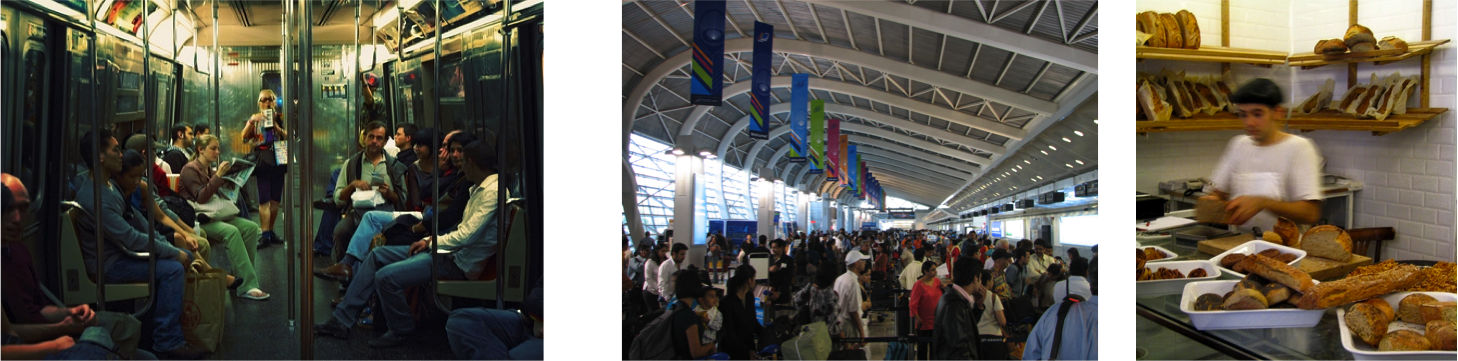
\includegraphics[width=3.5in]{images/people.png}
 \caption{Typical examples of scene categories from the SUN Dataset, containing varying numbers of people performing typical actions.}
 \label{fig:people}
\end{figure}

%One of the three core problems of computer vision, recognition has made long strides in the past years.  Accuracy of scene recognition algorithms has jumped, and HOG has practically become a household word.  But there is only so far that literal lines in an image can take recognition algorithms: these approaches can be brittle to camera angle and scale changes.

%One school of thought believes we should endeavor to make computer vision systems as similar to their human counterparts as possible; this means we need to consider what makes up a scene rather than how it is shaped.  This puts the onus of recognition on object detectors, which have also made noteworthy progress.

\section{Related work}

Weak features of oriented edge point histograms have long been used as image representations for applications such as object detection and scene recognition \cite{sift} \cite{gist}. Rather than using histograms as a global descriptor, stronger features can be composed by computing histograms of weak features on a dense grid of overlapping cells \cite{HOG}. Traditionally, these stronger features would be put into a ``bag of features'' and used as an orderless description of the image. However, scene categories can often be differentiated by their typical geometric organizations, and correspondence between images can be roughly computed by matching strong feature histograms of increasingly finer resolutions, as proposed by Lazebnik et. al. \cite{beyond_bags}. In this method, the image is repeatedly subdivided to create a spatial pyramid. Histograms of a dictionary of strong features are then matched level by level to compute the correspondence between two images. We extend upon this work by examining the use of spatial pyramids of different features. Additionally, we use spatial pyramids of strong features as a baseline with which we compare all the other methods we test. 

Spatial pyramids of strong features only capture the general organization of a scene, like the fact that the sky usually appears at the top of the image and the grass appears at the bottom. In order to capture the semantic meaning of image parts as well as their spatial organization, Li et. al. use spatial pyramids of the responses of a large number of object detectors \cite{object_bank}. This method takes into account the typical objects in a scene and their locations, but it does not give special significance to the appearance of people in the scene. We propose to augment this idea of scale invariant super-strong features by using spatial pyramids of the responses of people's locations and actions detectors. 	

In order to detect people in images and recognize the actions they are performing, Bourdev et. al. use part based detectors that operate on parts, or poselets, that are novel enough to allow for a correct detection of a whole person \cite{poselets}. While this technique requires hand annotation of several points per person for the learning phase, it performs impressively well as a person detector once trained. Additionally, poselets have been extended for use in determining people's activities, clothing, and gender \cite{poselets_actions}. We use poselets based person detectors as the super-strong features in our spatial pyramids.

Finally, the SUN Database is currently the most extensive dataset for scene recognition tasks as it contains 899 categories and 130,519 images \cite{SUN}. We use a subset of this dataset in all of our experiments in this project.


%The problem of scene recognition has been widely considered important by the computer vision community for many years.  The particular approach taken has varied over the years, but the general formula is to find the HOG of the image, split and combine it in ways that represent scales, location, and information importance, and use a histogram intersection kernel to build a one-vs-all SVM per scene category.  This is the approach taken by Lazebnik\ref{>>>>>??????<<<<<<<} ; she intends to localize features by organizing them into spatial pyramids.  That is, she takes an image, splits it in half in both dimensions, and repeats several times.  On each of these small parts, she does texton detection using a dictionary pre-constructed from 50 random images from her dataset.  She concatenates the texton histograms into one larger histogram.  She then retraces her steps: she performs texton detection on the larger-scale images and concatenates their histograms onto the formed histogram after penalizing them exponentially according to their scale.  This led to rather successful scene recognition on her fifteen category dataset.

%Beyond this, Feifei Li, et al., elected to follow in the direction of using knowledge about what's in a scene in order to identify it \cite{>>>>>>>>????????<<<<<<<}.  They reasoned that a toaster is more likely to be in a kitchen than at a harbor, and that we can leverage this humanesque knowledge to help our recognition task become easier.  Additionally, they applied, as we do, spatial pyramid organization to this object recognition: a boat is more likely to be found at the bottom of a frame and the sky is more likely to be found at the top, so those as features can be weighted appropriately.

%The other work that contributes directly to this endeavor is work on finding people in scenes.  The particular piece we consider is Bourdev's poselet work \ref{>>>>>??????<<<<<<<}.  Bourdev asserts that we are handicapping computers by allowing them only one image rather than a lifetime of experience in learning.  In order to approximate some part of this learning, he uses annotated images of people with ``key points'' marked: head, left shoulder, right shoulder, left hip, right hip, etc.  From these key point annotations, he groups similar annotation pieces (e.g. all people who are crossing their arms) and builds a classifier for each ``poselet'' described by these groups.  These classifiers work together to estimate key point locations and bounding boxes of people in an image.  Poselets have been extended for use in determining people's activities, clothing, and gender.


\section{Feature sets}

We composed two different scene recognition feature sets out of elements taken from pyramids of strong features and poselets \cite{poselets} \cite{beyond_bags}. Our first feature set uses Lazebnik et. al.'s spatial pyramids of strong features, together with the number of people in the image based on the poselets people detection algorithm. We threshold the poselet people detector with the recommended 5.7 confidence measure.
%For building texton dictionary - we took 200 centroids as was recommended in the papaer. We built the dictionary based on 50 randomly selected images from the training set again following her recommendation.

Our second feature set again uses spatial pyramids of strong features, but this time in conjunction with a separate set of spatial pyramids that records the locations and total counts of people in the image. To this end, we first run the poselet detector over the entire image to get the x,y locations, size and confidence level information for all the detected people in the image. We then use these people detector responses as features in a modified version of  Lazebnik et. al.'s algorithm. To build the pyramid we go from the finest to coarsest level. In each level and for each subregion we record the number of bounding boxes of people that fit entirely into the subregion but did not fit into a smaller contained subregion. Since we only count people that appear in recursively finer resolutions in the smallest resolution in which they are contained we do not need to penalize detections like in the original algorithm. We use a three level rather than a four level pyramid as the poselet detectors are limited in their ability to detect very small people, so subdividing the image any further did not increase performance.

We leave the addition of features based on people's actions in various locations to future work.

%We elected to build off of these two previously-published algorithms in creating our scene recognition feature set.  Bourdev and Lazebnik both made their code available for download on their websites, and we were able to run it with slight modifications relating to dataset location, aggregation, and caching settings.  We also composed these two algorithms into our pyramids of people algorithm.

%The pyramids of people algorithm tracks the spatial locations and total counts of people.  We first run Bourdev's poselets algorithm over the entire image to get x,y locations, size, and confidence level information for detected people in the image.  For thresholding, we elected to use the 5.7 confidence measure Bourdev chose for his poselet demonstration code.  We then co-opted the code for spatial pyramid formation from Lazebnik's code with a few modifications.

%We do not penalize people found at larger pyramid scales as Lazebnik penalized textons found at larger scales.  People found at larger scales are simply closer to the camera, and the scale information is valuable (imagine a scene of ten people regularly receding away from the camera in stadium seats at a ball game vs. a scene of ten people randomly milling about in a fast food restaurant).

%We also take into account the size of the people when determining which pyramid they belong in: Lazebnik considers textons to have an x,y position and no area in an image, while people have varying heights and widths that need to be accounted for.

%We also use fewer pyramid levels than Lazebnik does (3): one limitation of the poselets code in our experience is that it does not detect people smaller than a size of >>>>><<<<<<<??????, so it does not make sense to quarter the image more than three times.

\section{Data preprocessing}

Due to limited computing resources, we chose to first perform a proof of concept on 15 scene categories out of the full 908 category SUN dataset \cite{SUN}. Since our algorithm relies on the presence of people in the image we attempted to pick our scene categories wisely by sorting them by the number of images that contain people and picking the top 15 categories in the list.

To do this, we first manually identified all person-related object tags using the SUN Database online interface. We then picked the ``typical scenes'' where each of these object tags is most likely to appear. For each ``typical scene'', we aggregated the number of images tagged with any of the person-related object tag, and sorted the scene categories by this count. We then picked the top 15 categories in the list that contained at least 100 images, and used them in our experiments. From each one of our 15 scene categories, we randomly chose 50 images for training and 50 images for testing. These divisions were kept constant across all experiments. We plan to re-run our experiments with the full SUN dataset on a larger computer cluster.

%Due to the fact that we had only one machine to run our analysis on, we needed to cull the dataset somewhat.  The full SUN dataset is 131,072 images from 908 scene categories.  We had resources to train and test on approximately 50 images from 15 different scene categories owing to the long runtimes of both Lazebnik's spatial pyramid feature building and Bourdev's poselet detectors.  Since our algorithm relies on the presence of people, we wanted to choose scene categories with people present in them.

%On the website for the SUN database, CSAIL provides an interface for web users to tag objects in images.  One of the most prominently tagged object categories is ``person'' and derivatives like ``person standing'', ``person sitting'', and ``people''.  SUN offers ``typical scenes'' for each object category, which are the ten scene categories with the largest numbers of tags of that particular object category.  We aggregated the counts for all manually-identified ``person'' derivatives and ranked by largest number of tags.  We then eliminated scene categories with fewer than 100 images so that we would have at least 50 training images and 50 testing images available for each scene category.  From the remaining categories, we selected the 15 with the highest tag counts as our ``typical scenes.''

%We randomly split the images into 50 training and 50 testing images per scene category.  These divisions were kept constant across all experiments.

\section{Experiments}
We performed experiments using our clipped dataset with the two different feature sets we designed, and compared them to Lazebnick et. al.'s original spatial pyramid of strong features. Additionally, we conducted an ablation study in which we used only a spatial pyramid of people locations without the additional SIFT strong features.

In all cases we used the above-mentioned 50 training images to train a one-vs-all SVM classifier for each scene class, as described in Lazebnik et. al.'s paper. We used the LIBSVM library together with a histogram intersection kernel for classification, and tested our classifier on the full set of 50 test images per scene category \cite{libsvm}. Our experiments were performed on a quad core server, and the runtime was approximately 4 days.

\section{Results}

The following figures capture the results of our experiments. Figure \ref{fig:strong} depicts a baseline study where we only use spatial pyramids of strong features. Figure \ref{fig:poselets_strong} depicts an experiment where we add the total number of people in the image as a feature. This addition did not improve the recognition accuracy, but resulted in a slightly different confusion matrix. In Figure \ref{fig:pyramid_poselets_strong} we explore the usage of spatial pyramids of people detections in addition to strong features. As a sanity check, we perform an ablation test where we only use spatial pyramids of people detections. Figure \ref{fig:pyramid_poselets_only} demonstrates that this feature alone did not perform well in our experiment.

\begin{figure}[p]
 \centering
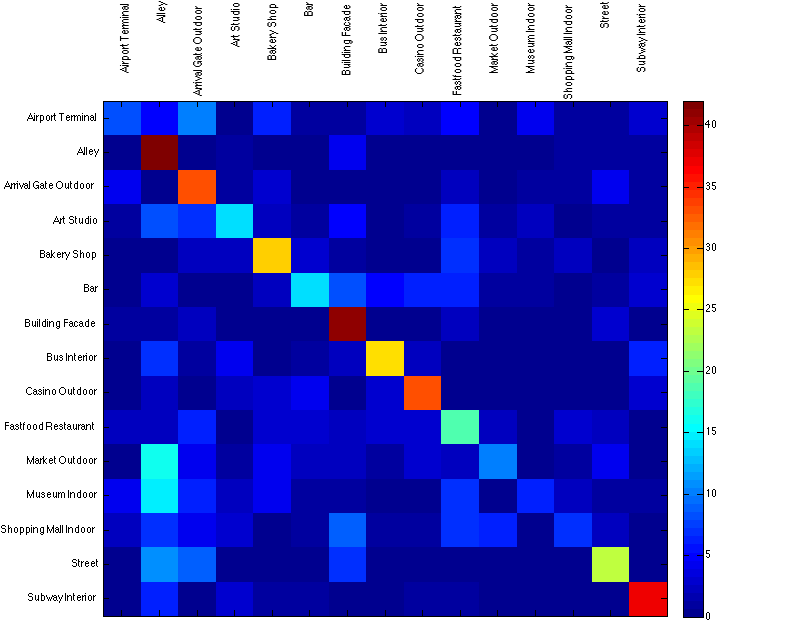
\includegraphics[width=3.5in]{images/Strong_features.png}
 \caption{A baseline experiment using Lazebnik et. al.'s original spatial pyramids of strong features algorithm together with our dataset. Accuracy is 0.456.}
 \label{fig:strong}
\end{figure}

\begin{figure}[p]
 \centering
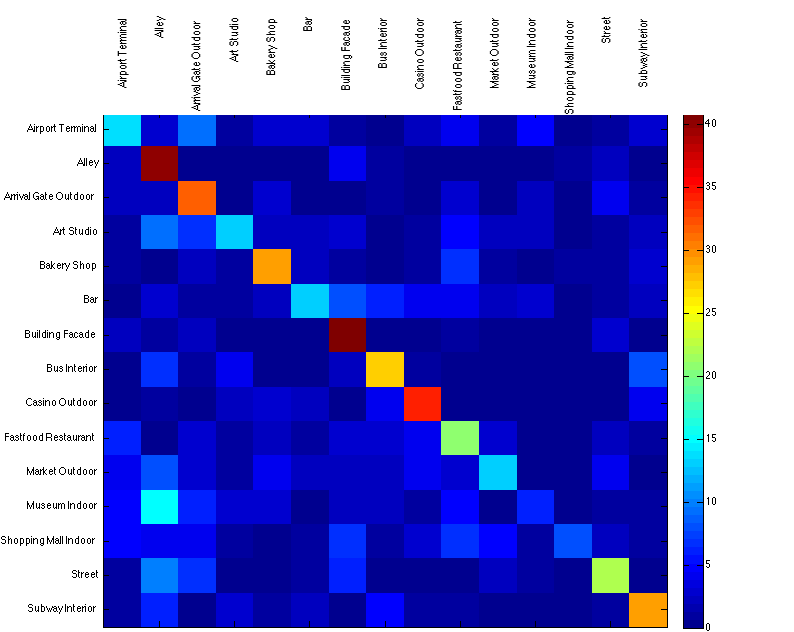
\includegraphics[width=3.5in]{images/Poselets_and_strong_features.png}
 \caption{Spatial pyramids of strong features plus a feature depicting the count of people in each image, without any spatial information. Accuracy is 0.456.}
 \label{fig:poselets_strong}
\end{figure}

\begin{figure}[p]
 \centering
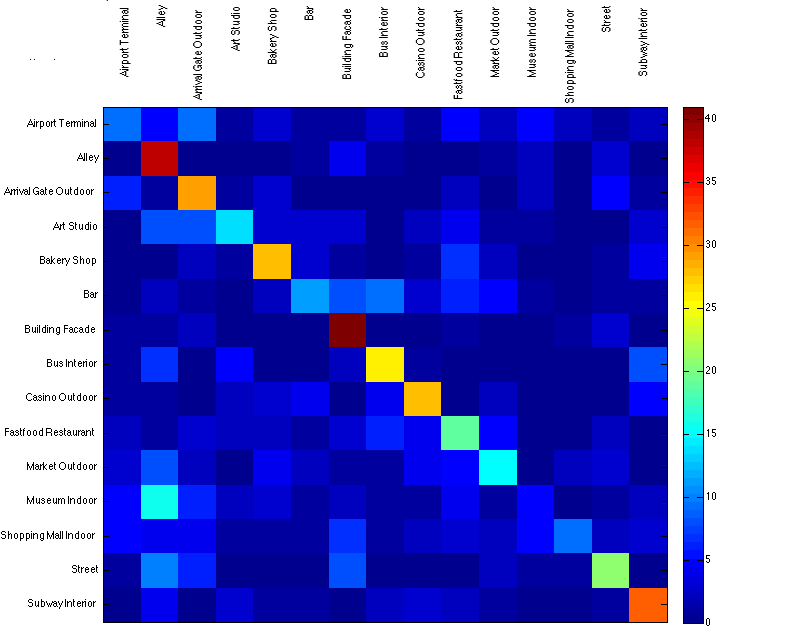
\includegraphics[width=3.5in]{images/Pyramid_poselets_and_strong_features.png}
 \caption{Spatial pyramids of strong features plus spatial pyramids of people detections. Accuracy is 0.433.}
 \label{fig:pyramid_poselets_strong}
\end{figure}

\begin{figure}[p]
 \centering
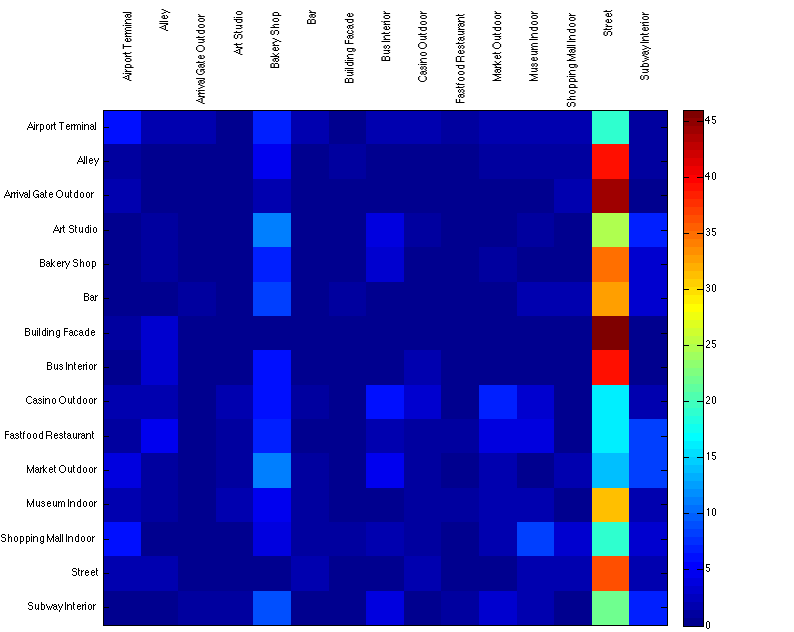
\includegraphics[width=3.5in]{images/pyramid_poselets_only.png}
 \caption{An ablation study in which we used only the spatial pyramids of people without strong features. Accuracy is 0.089.}
 \label{fig:pyramid_poselets_only}
\end{figure}

\section{Discussion}

We hypothesized that the distribution of people in scenes would be a discriminating feature that would enable correct classification of scene categories. Moreover, we expected that the addition of this feature would improve upon the original spatial pyramids of strong features. Neither of these expectations were fulfilled in our results. This may be due to the small size of our dataset, due to a suboptimal parameter selection, or due to the way we recursively split the images to create spatial pyramids. When subdividing images, we currently use Lazebnik et. al.'s original algorithm that cuts the image down the middle on every split. This may not be the best choice, as according to the rules of good photography it is often common to place the horizon line at the center of the image. This would cause all the bounding boxes of people that intersect the horizon to not completely fit into any by the coarsest scale of our pyramid, resulting in incorrect counts in all other scales.

\section{Future Work}
We would like to continue investigating the potential of the distribution of people in images as a feature for scene recognition.  We plan to test on a larger cluster in the next week with the full SUN dataset.  We would also like to examine the power of the poselet attribute work (determining gender, activity, and clothing) on our work.  Intuitively, a scene in which many people seem to be riding horses is more likely to be a rodeo than a scene in which many people seem to be lying down.

\bibliographystyle{plain}
\bibliography{report}
\end{document}
